\section*{Dag 6. 12-01-2026}
\vspace{1em}

I dag har vi fået lavet: 
\begin{itemize}
    \setlength{\itemsep}{3pt}
    \setlength{\parskip}{0pt}
    \setlength{\parsep}{0pt}
  \item et udkast til flowdiagram
  \item Box diagram
  \item Valgt kravspecifikationer 
  \item Et gantt chart
\end{itemize}

\textbf{Flowchart}

\begin{figure}[h]
    \centering    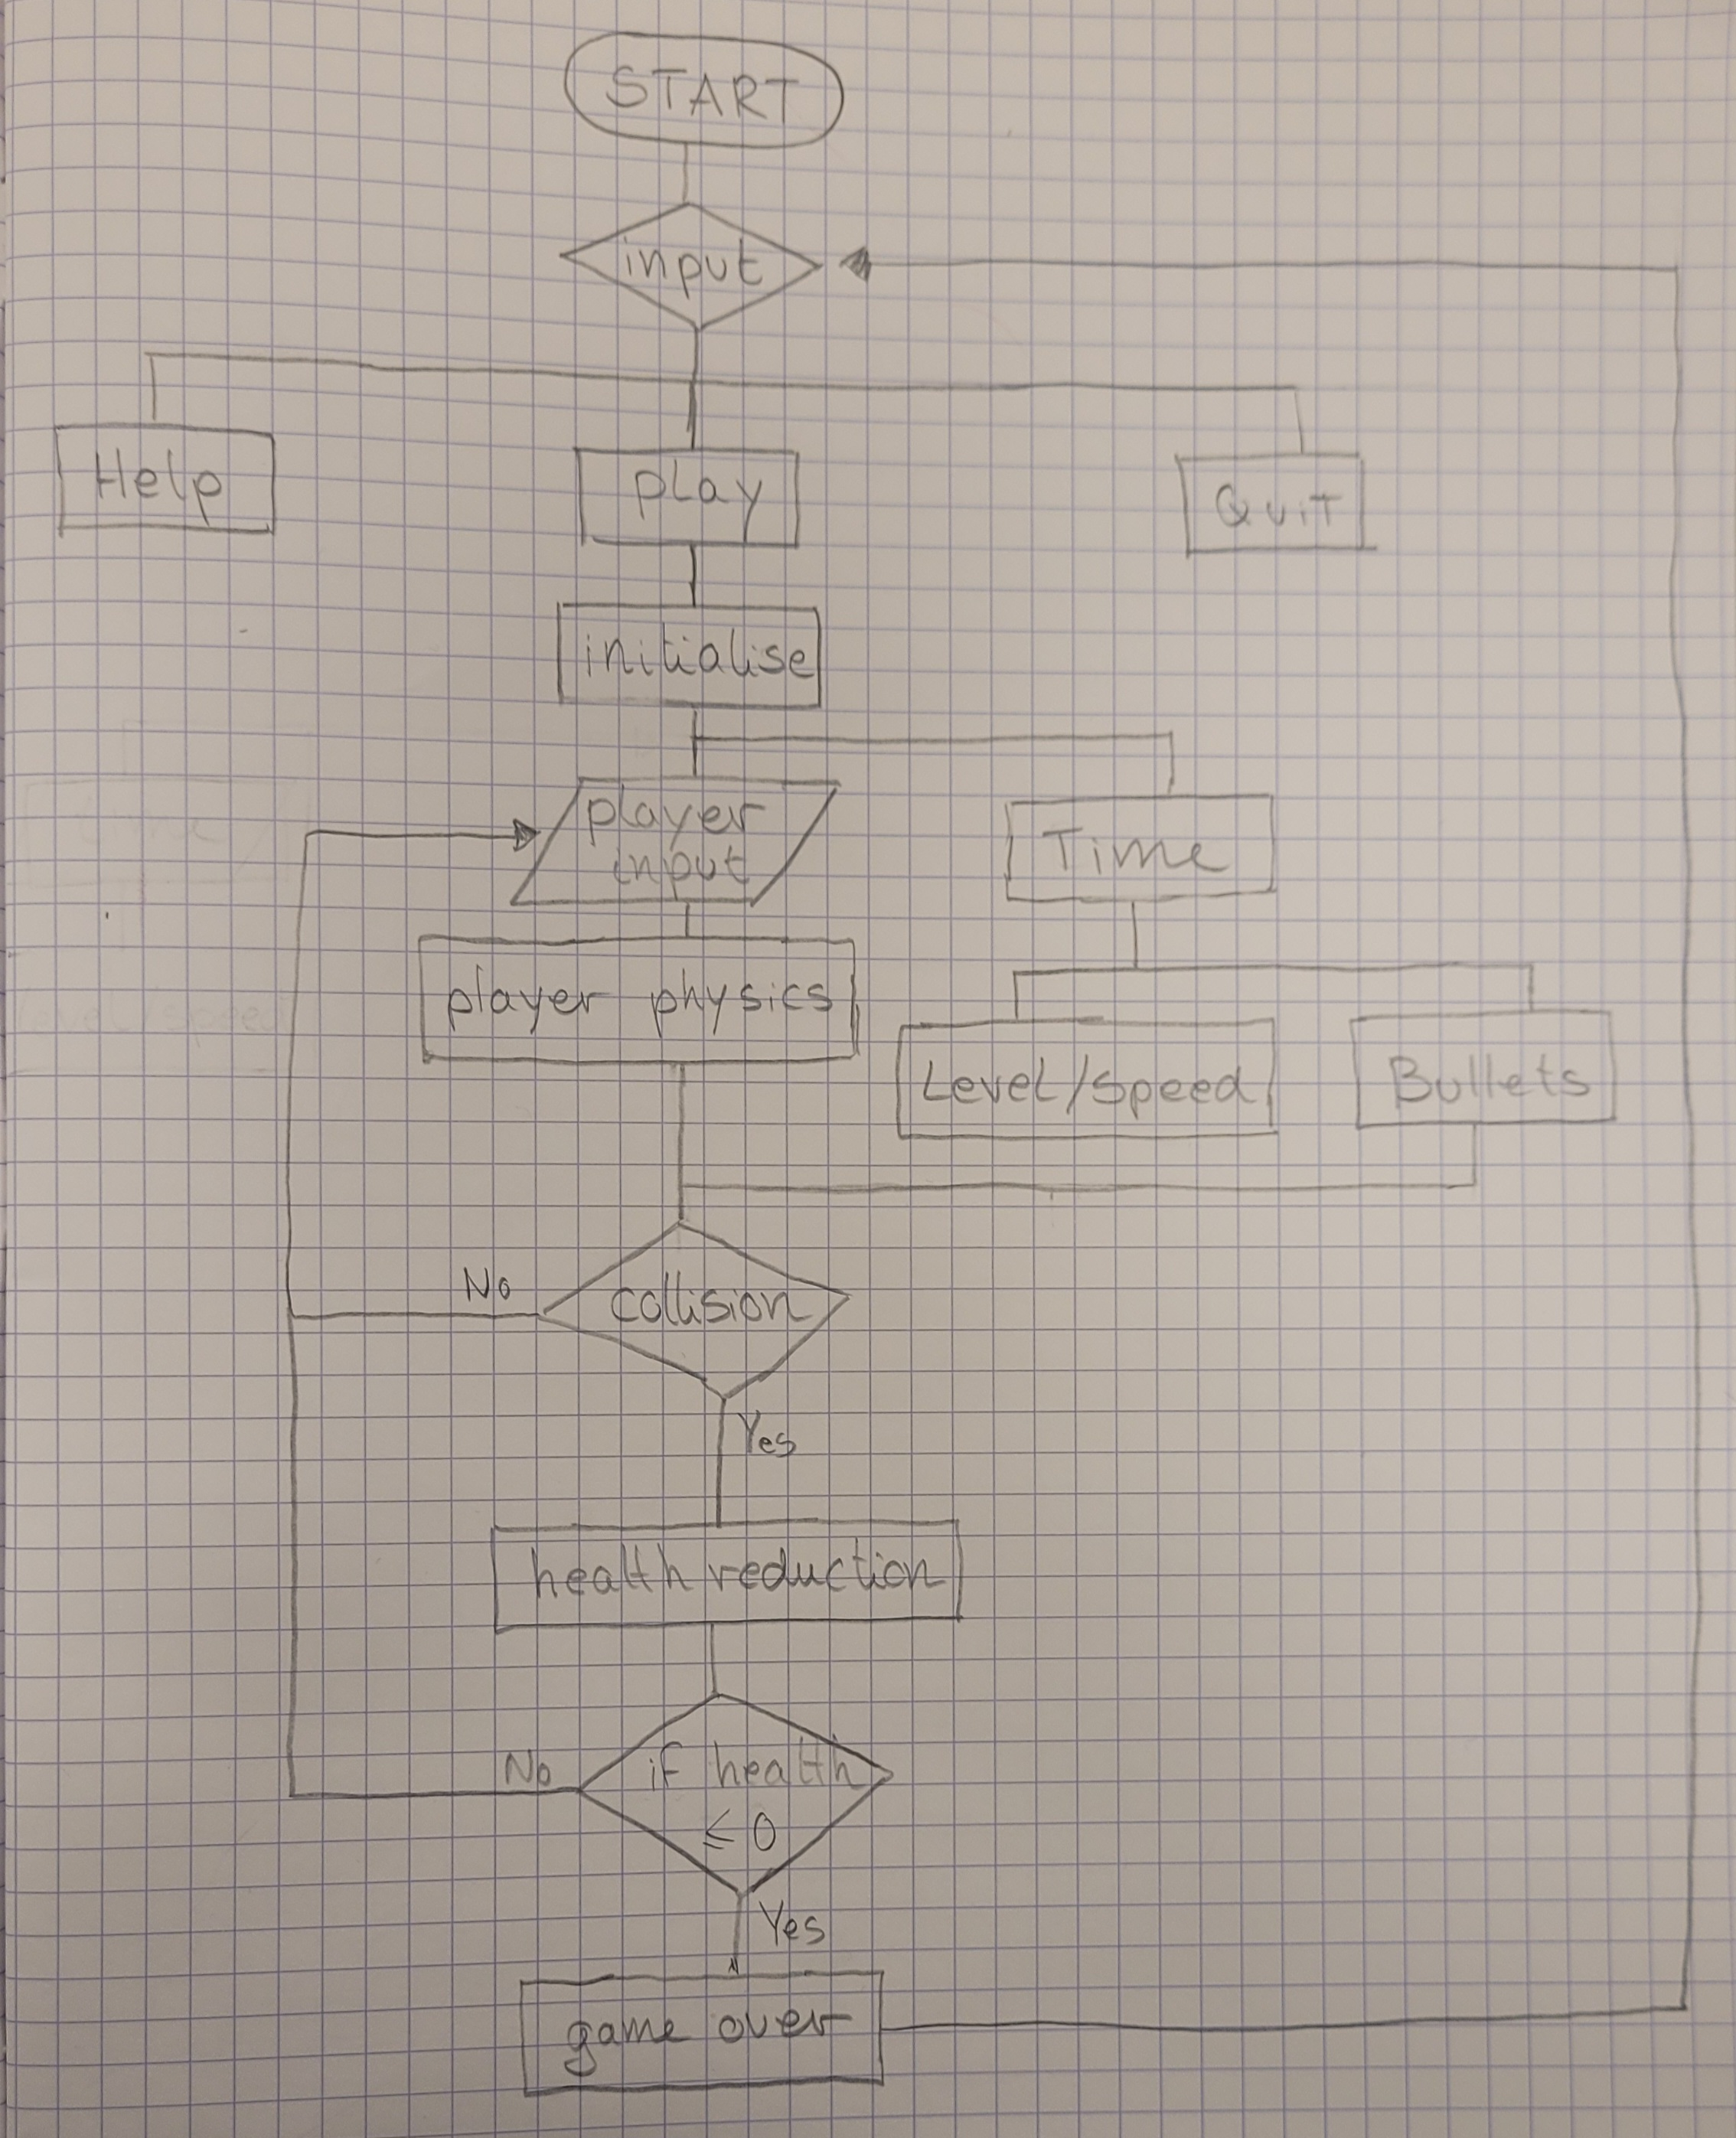
\includegraphics[width=0.9\textwidth]{Picturs/Journal/20260112_160159.jpg}
    \caption{Udkast til Flowdiagram}
\end{figure}

\vspace{4em}

\textbf{Box diagram}

\begin{figure}[h]
    \vspace{-1em}
    \centering  
    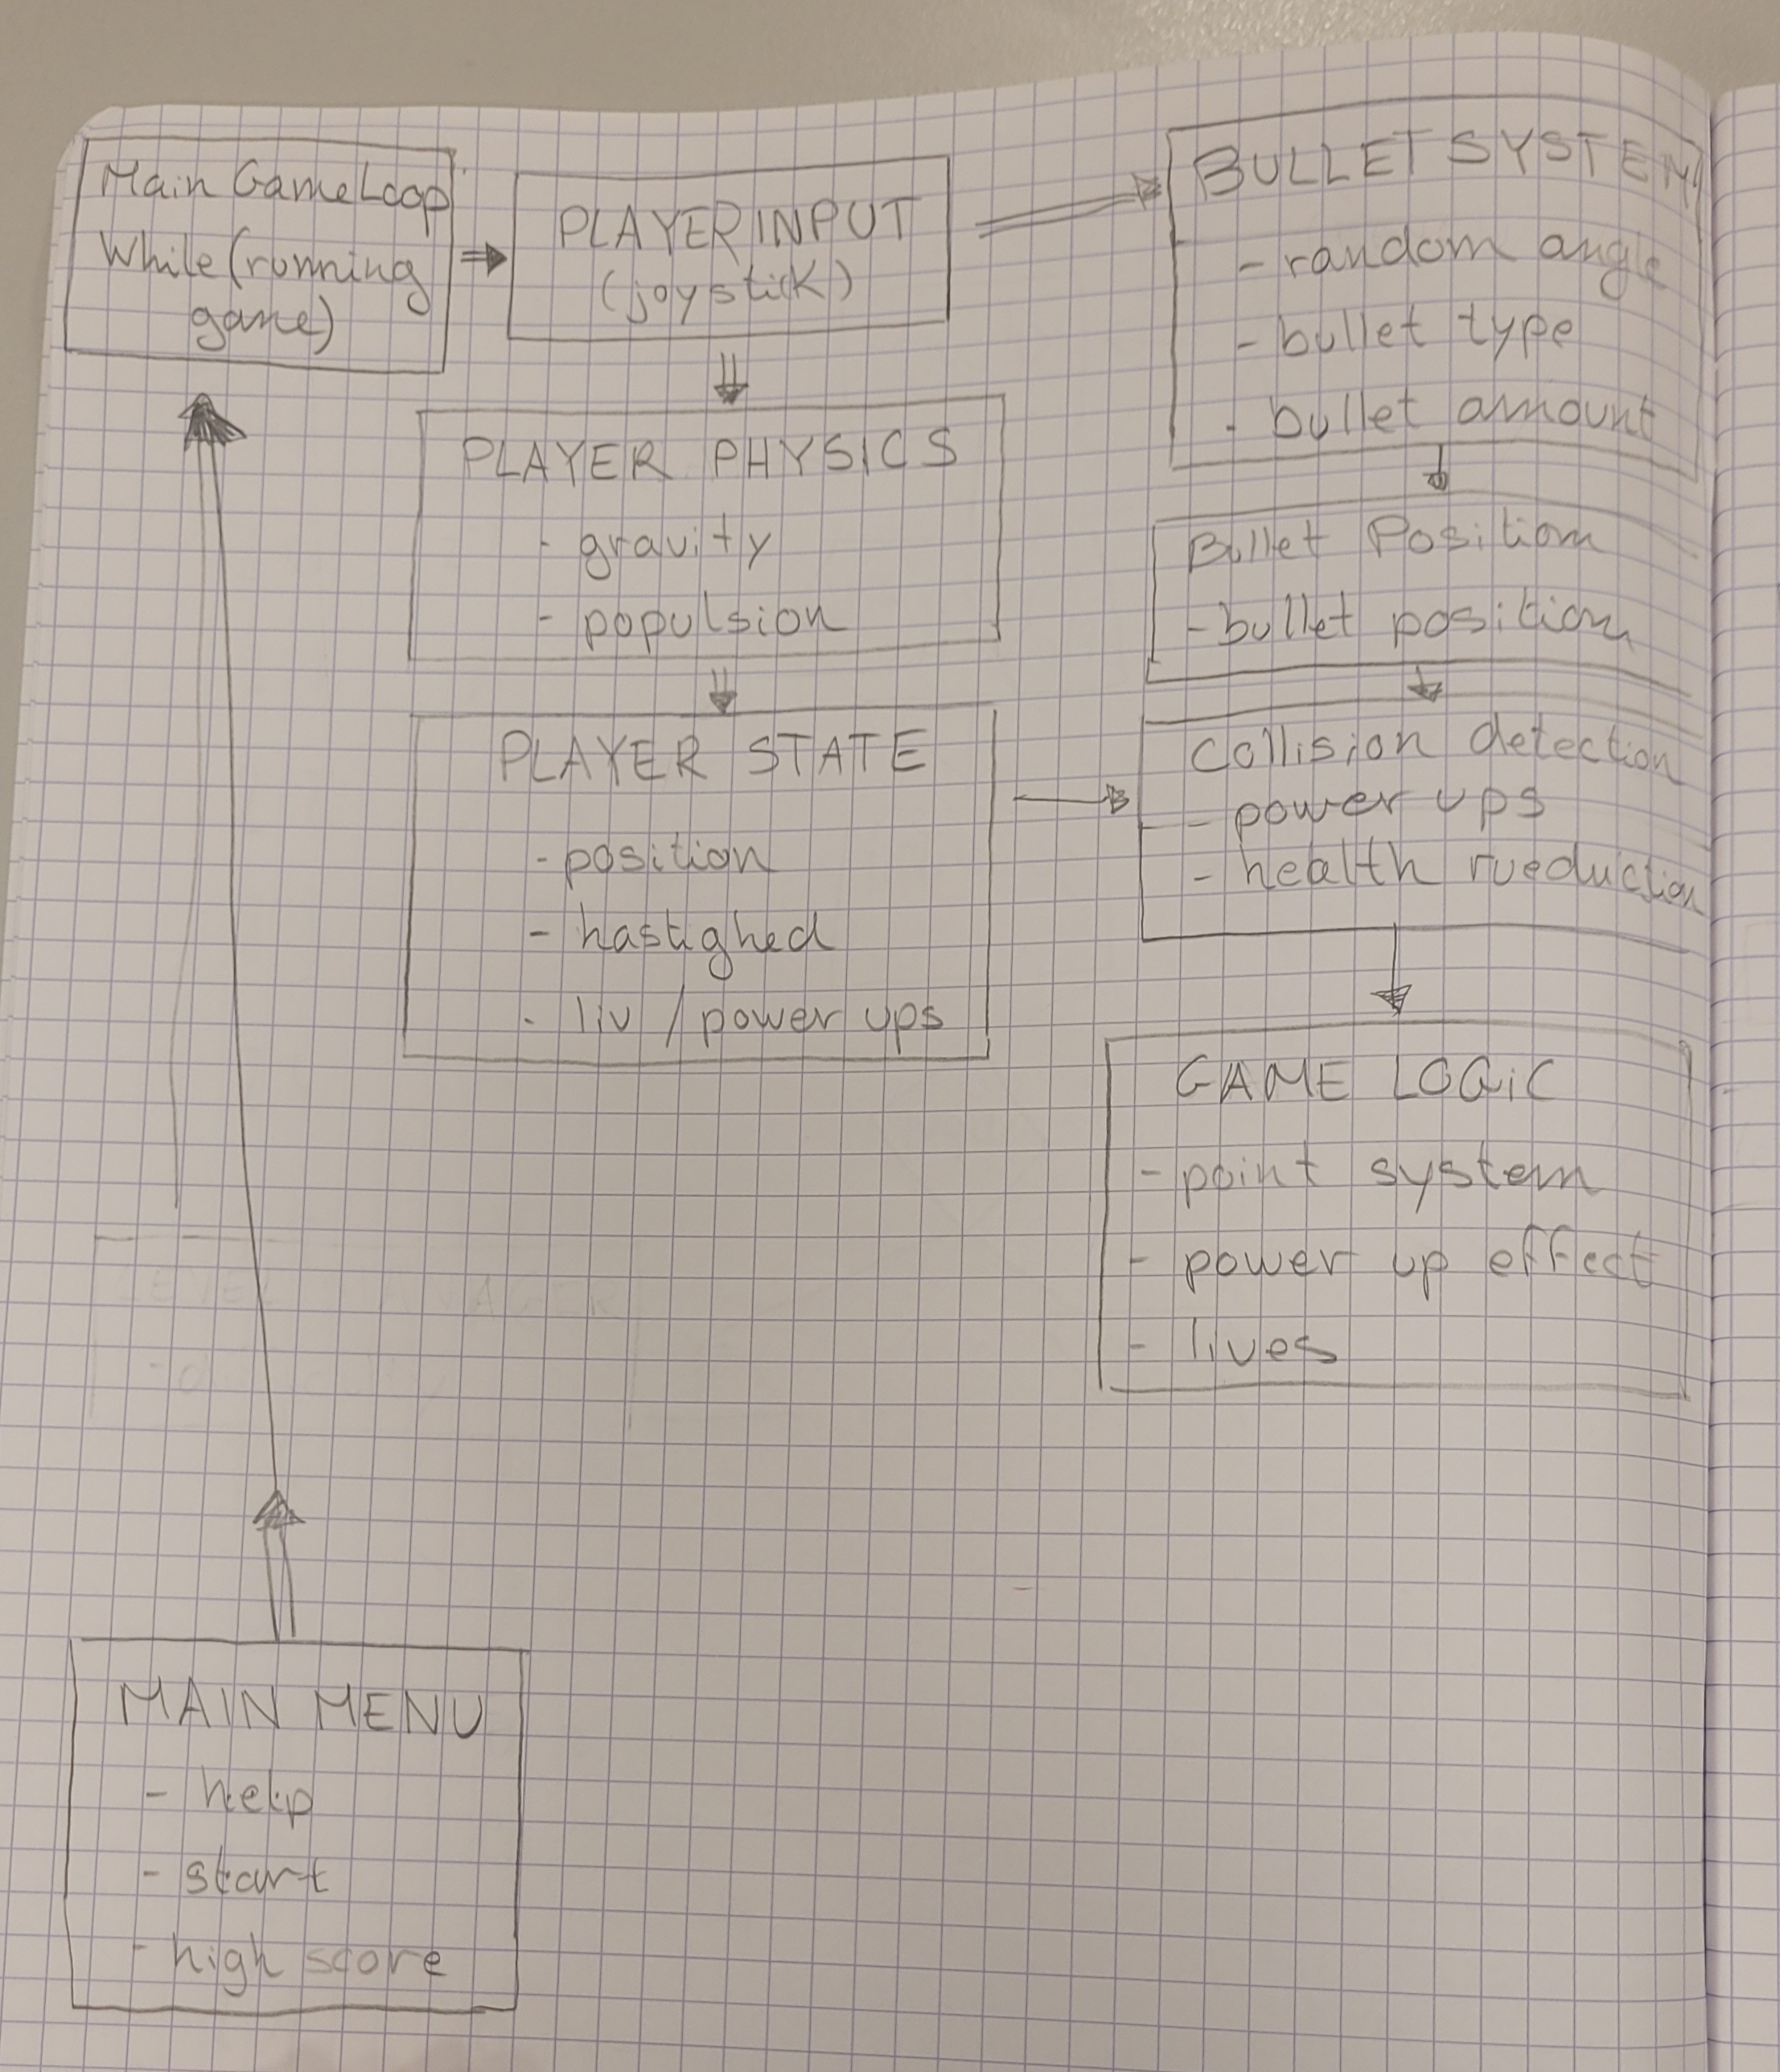
\includegraphics[width=0.7\textwidth]{Picturs/Journal/20260112_160243.jpg}
    \caption{Udkast til block diagram}
    \vspace{-1em}
\end{figure}

\textbf{Gantt chart}

\begin{figure}[h]
    \vspace{-1em}
    \centering    
    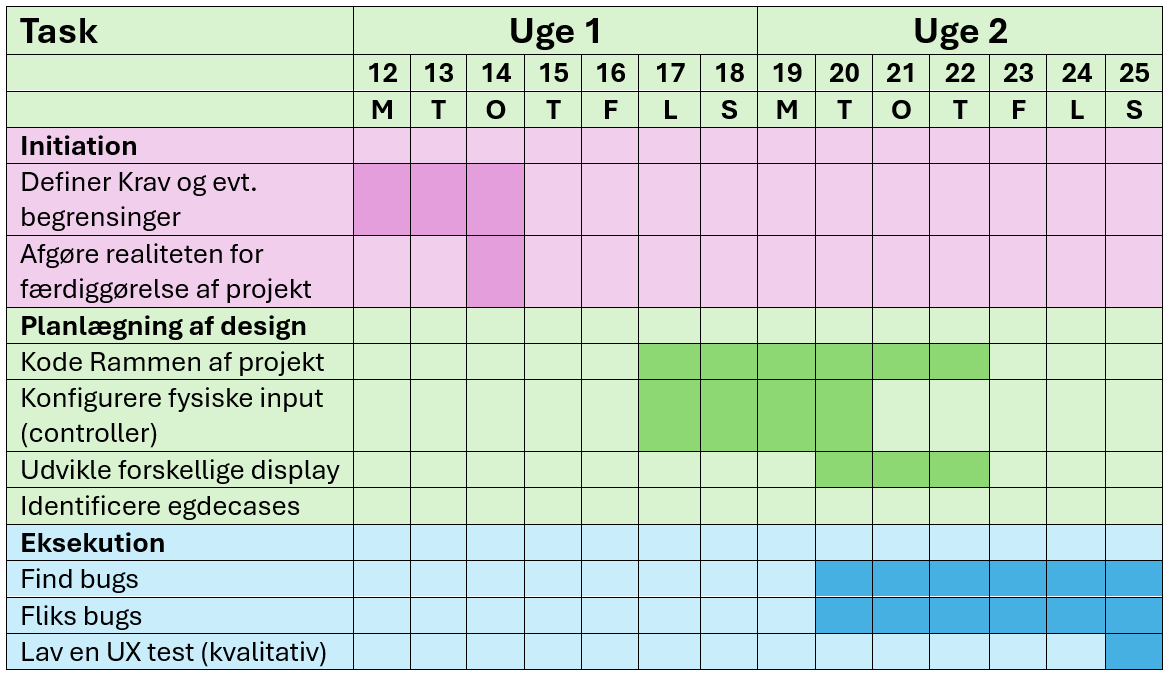
\includegraphics[width=1\textwidth]{Picturs/Journal/gantchart.png}
    \caption{Udkast til Gantt Chart}
    \vspace{-10em}
\end{figure}

\vspace{8em}

\textbf{Valgte kravspesifikationer}

\begin{table}[h!]
\centering
\begin{tabularx}{\textwidth}{|l|X|}
\hline
\textbf{Det vi skal have med} & \textbf{Uddybelse} \\
\hline
Asteroider/planeter med potential felt & no \\
\hline
3+ stages docked spaceships & There are multiple levels (faster, more and different types of bullets) \\
\hline
3+ bullet types + 5+ shot angles & Types of bullets include:
\begin{itemize}[leftmargin=*]
    \item regular bullet: 1 dmg, size: medium (“\%c”,220), speed: medium
    \item bouncing bullet: 1 dmg, size: medium, speed: medium (“\%c”,220) (shot so it hits the wall and bounces)
    \item cannon ball: 2 dmg, size: large 2*(“\%c”,219), speed: slow
    \item sniper bullet: 3 dmg, size: small (“\%c”,254), speed: fast (maybe targeted at player position?)
\end{itemize} \\
\hline
Power-ups & powerups including healing, point multiplier for a time period, some sort of forcefield (outward acceleration or deflection of bullets) \\
\hline
Number of points & point i forhold til tid \\
\hline
Multiple lives & x antal liv som du mister indtil antal liv er x $\leq 0$, og du dør \\
\hline
Menu & 
\begin{itemize}[leftmargin=*]
    \item Help button
    \item Play button
    \item High score
    \item Level (sværhedsgrad)
\end{itemize}
Selected button indikeres af anti characters på given button \\
\hline
Help screen & controls, how to play \\
\hline
Boss key & Brings up a menu displaying the buttons: resume, main menu, help \\
\hline
Random delta-angle & den vinkel “fjenden” skyder med \\
\hline
Multiple bullet & dem som “fjenden” skyder med / meteore \\
\hline
Score / high score & 
\begin{itemize}[leftmargin=*]
    \item displays på LCD
    \item øges med til og evt. powerups
\end{itemize} \\
\hline
Game controlled by 30010 joystick & 
\begin{itemize}[leftmargin=*]
    \item klik: så længe du holder den nede flyver du op
    \item up/down/left/right: bruges måske i menuen
\end{itemize} \\
\hline
Show info on RGB LED &
\begin{itemize}[leftmargin=*]
    \item spil slukket: ingen lys
    \item spil tændt - ikke aktivt: hvid
    \item mens du spiller: grøn
    \item mister et liv: blinker kort i rød
    \item død: rød
\end{itemize} \\
\hline
Partial/full game on the LCD &
\begin{itemize}[leftmargin=*]
    \item displayer løbende score
    \item display af highscore
    \item display af antal liv
\end{itemize}
\end{tabularx}
\end{table}

